\documentclass[12pt]{article}
\usepackage{etoolbox}
\usepackage{listings}
\usepackage{float}
\usepackage{graphicx}
\usepackage{color}
\usepackage[justification=centering]{caption}
\usepackage{hyperref}


\hypersetup{
	colorlinks,
	citecolor=black,
	filecolor=black,
	linkcolor=black,
	urlcolor=black
	}

\setcounter{secnumdepth}{4}
\setcounter{tocdepth}{4}

\definecolor{mygreen}{rgb}{0,0.6,0}
\definecolor{mygray}{rgb}{0.5,0.5,0.5}
\definecolor{mymauve}{rgb}{0.58,0,0.82}

\lstset{ %
	backgroundcolor=\color{white},   % choose the background color; you must add \usepackage{color} or \usepackage{xcolor}
	basicstyle=\footnotesize,        % the size of the fonts that are used for the code
	breakatwhitespace=false,         % sets if automatic breaks should only happen at whitespace
	breaklines=true,                 % sets automatic line breaking
	captionpos=b,                    % sets the caption-position to bottom
	commentstyle=\color{mygreen},    % comment style
	deletekeywords={...},            % if you want to delete keywords from the given language
	escapeinside={\%*}{*)},          % if you want to add LaTeX within your code
	extendedchars=true,              % lets you use non-ASCII characters; for 8-bits encodings only, does not work with UTF-8
	%	frame=single,                    % adds a frame around the code
	keepspaces=true,                 % keeps spaces in text, useful for keeping indentation of code (possibly needs columns=flexible)
	keywordstyle=\color{blue},       % keyword style
	language=[Motorola68k]Assembler, % the language of the code
	morekeywords={*,...},            % if you want to add more keywords to the set
	numbers=left,                    % where to put the line-numbers; possible values are (none, left, right)
	numbersep=5pt,                   % how far the line-numbers are from the code
	numberstyle=\small\color{mygray}, % the style that is used for the line-numbers
	rulecolor=\color{black},         % if not set, the frame-color may be changed on line-breaks within not-black text (e.g. comments (green here))
	showspaces=false,                % show spaces everywhere adding particular underscores; it overrides 'showstringspaces'
	showstringspaces=false,          % underline spaces within strings only
	showtabs=false,                  % show tabs within strings adding particular underscores
	stepnumber=1,                    % step between two line-numbers. If it's 1, each line will be numbered
	stringstyle=\color{mymauve},     % string literal style
	tabsize=2                  % sets default tabsize to 2 spac                  % show the filename of files included with \lstinputlisting; also try caption instead of title
}
\makeatletter
\patchcmd{\l@section}
{\hfil}
{\leaders\hbox{\normalfont$\m@th\mkern \@dotsep mu\hbox{.}\mkern \@dotsep mu$}\hfill}
{}{}
\makeatother
\begin{document}
	
	\begin{titlepage}
		
		\newcommand{\HRule}{\rule{\linewidth}{0.5mm}} % Defines a new command for the horizontal lines, change thickness here
		
		\center % Center everything on the page
		
		%----------------------------------------------------------------------------------------
		%	HEADING SECTIONS
		%----------------------------------------------------------------------------------------
		
		\textsc{\LARGE Illinois Institute of Technology}\\[1.5cm] % Name of your university/college
	%	\textsc{\Large Major Heading}\\[0.5cm] % Major heading such as course name
		%\textsc{\large Minor Heading}\\[0.5cm] % Minor heading such as course title
		
		%----------------------------------------------------------------------------------------
		%	TITLE SECTION
		%----------------------------------------------------------------------------------------
		
		\HRule \\[0.4cm]
		{ \huge \bfseries ECE 441 Monitor Project}\\[0.4cm] % Title of your document
		\HRule \\[1.5cm]
		
		%----------------------------------------------------------------------------------------
		%	AUTHOR SECTION
		%----------------------------------------------------------------------------------------
		
		\begin{minipage}{0.4\textwidth}
			\begin{flushleft} \large
				\emph{Author:}\\
				Adam \textsc{Sumner} % Your name
			\end{flushleft}
		\end{minipage}
		~
		\begin{minipage}{0.4\textwidth}
			\begin{flushright} \large
				\emph{Teaching Assistant:} \\
				Boyang \textsc{Wang} % Supervisor's Name
			\end{flushright}
		\end{minipage}\\[4cm]
		
		% If you don't want a supervisor, uncomment the two lines below and remove the section above
		%\Large \emph{Author:}\\
		%John \textsc{Smith}\\[3cm] % Your name
		
		%----------------------------------------------------------------------------------------
		%	DATE SECTION
		%----------------------------------------------------------------------------------------
		
		{\large April 28th, 2015}\\[3cm] % Date, change the \today to a set date if you want to be precise
		
		%----------------------------------------------------------------------------------------
		%	LOGO SECTION
		%----------------------------------------------------------------------------------------
		
		%\includegraphics{Logo}\\[1cm] % Include a department/university logo - this will require the graphicx package
		
		%----------------------------------------------------------------------------------------
		
		\vfill % Fill the rest of the page with whitespace
		
		\textbf{Acknowledgment} \\ \flushleft I acknowledge all of the work including figures and code belongs to me and/or persons who are referenced.
	\end{titlepage}
	
	\tableofcontents
	\newpage
	\listoffigures
	\newpage
	\addtocontents{toc}{~\hfill\textbf{Page}\par}
	%\chapter{...}
	\begin{abstract}
		This project involved designing and implementing a Monitor program using the MC68000 assembly language. The program implements twelve basic debugger functions as well as two author defined functions. It is designed to handle exceptions, and is meant to be an educational piece of software for students taking ECE 441 at the Illinois Institute of Technology.
	\end{abstract}
	
	\section{Introduction}
	The \textsc{Sanper-1 ELU} is a Motorola MC68000 based microcomputer designed by Dr. Jafar Saniie and Mr. Stephen Perich for use in college level computer engineering courses\cite{manual}. For user interaction, it utilizes a monitor program called TUTOR that enables users to actively interact with the microcomputer. The design objective of this project is to re-implement the functionality of TUTOR into a student written monitor program titled MONITOR441. The program should be able to perform basic debugger functions such as memory display, memory sort, memory change, etc., and must have the ability to handle exceptions. The design constraints are:
	\begin{itemize}
		\item Code must be smaller that 3K starting from address \$1000
		\item Stack size must be 1K starting at memory location \$3000
		\item Macros may not be used
		\item Erroneous inputs should not kill the program
	\end{itemize}
	Twelve debugger functions must be implemented, along with two user defined debugger commands.
	
	\section{Monitor Program}
	The monitor program operates in a command driven environment. It acts as a typical shell, providing a user interface to access the microcomputer's services. The main program being run is a command line interpreter. Based on the input that the user enters, the interpreter determines if the input entered is valid and subsequently executes the specified command. It was developed using the Easy68K Simulator, thus the TRAP \#15 handler is used instead of the MC68000's TRAP \#14 handler. The structure of how this program operates is shown in Figure \ref{fig:monitor}.
		\begin{figure}[H]
			\centering
			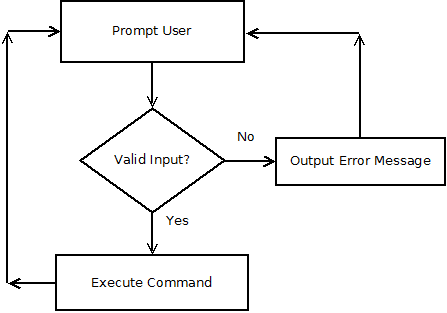
\includegraphics[width=0.7\linewidth]{monitor.png}
			\caption{Structure of Monitor Program}
			\label{fig:monitor}
		\end{figure}
		
		\subsection{Command Interpreter}
			\subsubsection{Algorithm and Flowchart}
			The algorithm for the command interpreter uses simple string matching to determine if input is correct. The algorithm begins by outputting the message \texttt{MONITOR441>} and accepting input from the user. It then checks for the ASCII value \$48 which corresponds to the letter H. This is to check for either the \texttt{HELP} command or \texttt{HXDC} command. If an H was not entered, it then checks for the ASCII value \$4D which corresponds to a memory command. If this fails, then it checks for ASCII value \$47, corresponding to the \texttt{GO} command. If this fails, the ASCII value \$44 is tested, corresponding to the \texttt{DF} command. If this fails, it checks for \$42, which signifies a \texttt{BLCK} command. If this fails, \$53 is tested for the \texttt{SORTW} command. If this fails, \$45 is tested for the \texttt{ECHO} command. If this fails \$2E is checked for the modify register command. If all of these checks fail, the user has entered incorrect input and an error message is displayed. If any of these checks succeed, the command line interpreter jumps to the respective command's helper interpreter function. These subroutines check for each character of the user input in order to verify the command the user entered was correct. These helper functions also serve to differentiate commands that start with the same character. The flowchart for this process is shown in Figure \ref{fig:commandint}.
			
			\begin{figure}[H]
				\centering
				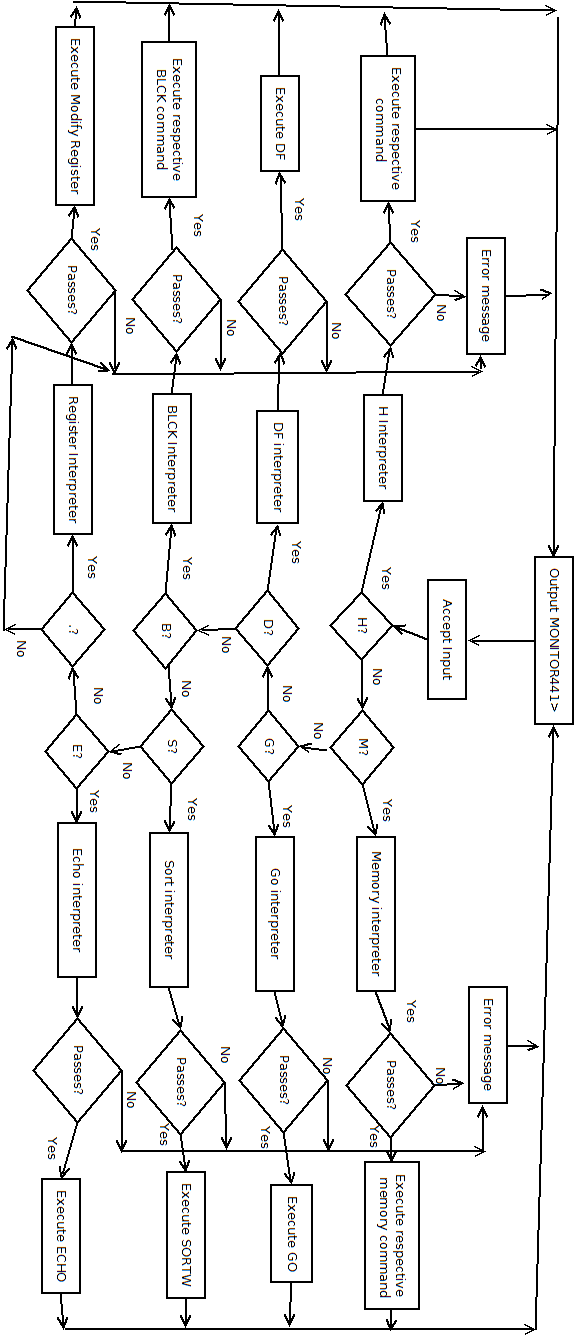
\includegraphics[width=.55\linewidth]{commandint}
				\caption{Flowchart for Command Line Interpreter}
				\label{fig:commandint}
			\end{figure}
			
			\subsubsection{Assembly Code}
			\lstinputlisting[firstline=154,lastline=412,firstnumber=154]{Project.X68}
			
			\subsection{Debugger Commands}
			\subsubsection{Help}
			\paragraph{Algorithm and Flowchart}~\\
			Help is a simple command that prints out a series of strings that display the available commands, their syntax, and a short description of each command. The syntax to invoke this command is \texttt{HELP}. The flowchart for this command is shown in Figure \ref{fig:help}.
			
			\begin{figure}[H]
				\centering
				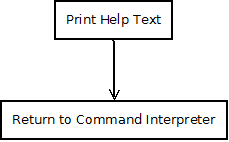
\includegraphics[width=0.4\linewidth]{help}
				\caption{Flowchart for Help}
				\label{fig:help}
			\end{figure}
			
			\paragraph{Assembly Code}~\\
			\lstinputlisting[firstnumber=797,firstline=797,lastline=983]{Project.X68}
			\subsubsection{Memory Display}
			\paragraph{Algorithm and Flowchart}~\\
			Memory display is an extremely useful tool to look at blocks of memory. The syntax to call this function is \texttt{MDSP <address1> <address2}, where \texttt{<address1>} is the starting address and \texttt{<address2>} is the ending address of the memory contents to be shown. This command also displays the block of memory from \texttt{<address1>} to \texttt{<address2 +16bytes>}. The flowchart for this command is shown in Figure \ref{fig:memdsp}.
				
			\begin{figure}[H]
				\centering
				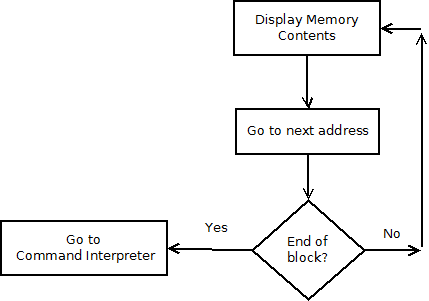
\includegraphics[width=.7\linewidth]{memdsp}
				\caption{Flowchart for Memory Display}
				\label{fig:memdsp}
			\end{figure}
			
			\paragraph{Assembly Code}~\\
			\lstinputlisting[firstnumber=1034,firstline=1034,lastline=1092]{Project.X68}
			
			\subsubsection{HXDEC}
			\paragraph{Algorithm and Flowchart}~\\
			This command allows the user to enter a hexadecimal value (up to FFFF), and the program will return the equivalent value in decimal format. The syntax to call this function is \texttt{HXDEC <data>}. It works by extracting the ASCII values byte by byte and determining the 16's place of each byte. The value extracted is then multiplied by its respective 16's place and added to a register that stores the total. This total must then be converted into BCD for output and then into ASCII to display it on the terminal. The flowchart for this command is shown in Figure \ref{fig:HXDEC}.
			
			
\begin{figure}[H]
\centering
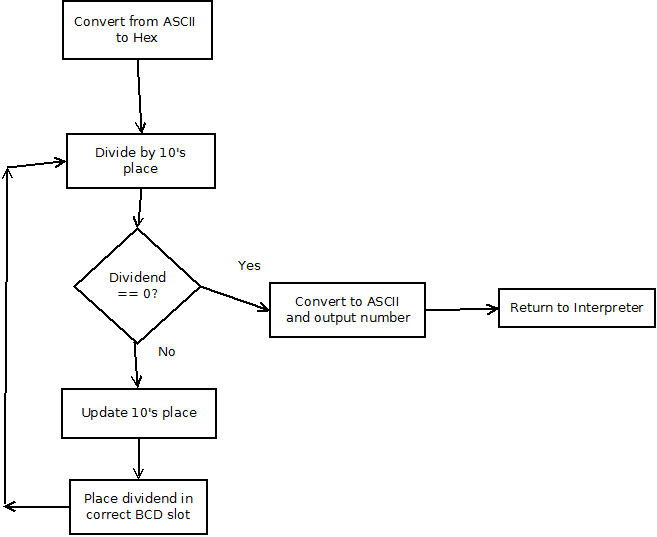
\includegraphics[width=0.7\linewidth]{HXDEC}
\caption{Flowchart for HXDEC}
\label{fig:HXDEC}
\end{figure}
			\paragraph{Assembly Code}~\\
			\lstinputlisting[firstnumber=1096,firstline=1096,lastline=1155]{Project.X68}
			
			\subsubsection{SORTW}
			
			\paragraph{Algorithm and Flowchart}~\\
			This command implements the most common sort algorithm for a set of data, the bubble sort. Because the user has the choice to choose between sorting the data in ascending or descending order, it also implements a ``rock" sort. It works by first determining which option, ascending or descending, the user has selected. Once determined, the first data in the set is analyzed to the next immediate adjacent value in memory. If the current data is larger than the next data (assuming ascending order for example), the two words of data are swapped. This value is continuously checked against its immediate adjacent memory until it ``fits" in the current state of the list. This process is repeated for n elements in a list of n words. The runtime is $\mathcal{O}(n^2)$, and the syntax for this command is \texttt{SORTW <option> <address1> <address2>}, where both \texttt{<address1>} and \texttt{<address2>} are even addresses. The flowchart is shown in Figure \ref{fig:SORTW}.
			
			
\begin{figure}[H]
\centering
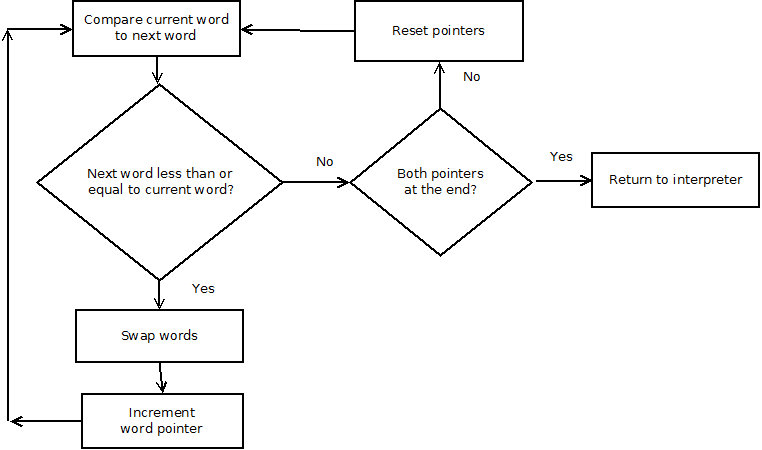
\includegraphics[width=0.7\linewidth]{SORTW}
\caption{Flowchart for SORTW}
\label{fig:SORTW}
\end{figure}
			\paragraph{Assembly Code}~\\
			\lstinputlisting[firstnumber=1159,firstline=1159,lastline=1278]{Project.X68}
			
			\subsubsection{Memory Modify}
			
			\paragraph{Algorithm and Flowchart}~\\
			This command first determines which option the user has selected. Depending on this option, it reads the address entered by the user and displays the specified amount of data currently stored in memory. The user is then prompted to enter data to store into memory. The command increments the memory location and asks for input until the user enters the '.' character. The syntax for this command is \texttt{MM <option> <address>}. The flowchart is shown in Figure \ref{fig:MM}.
			
\begin{figure}[H]
\centering
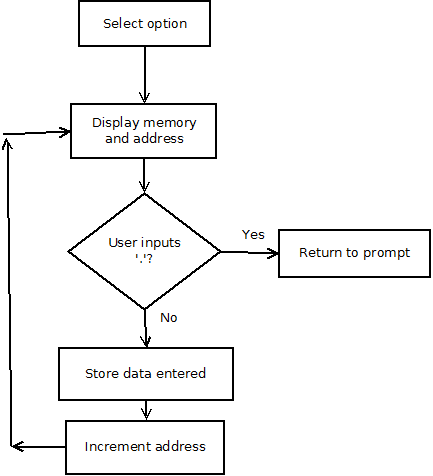
\includegraphics[width=0.7\linewidth]{MM}
\caption{Flowchart for Memory Modify}
\label{fig:MM}
\end{figure}
			\paragraph{Assembly Code}~\\
			\lstinputlisting[firstnumber=1282,firstline=1282,lastline=1622]{Project.X68}
			
			\subsubsection{Memory Set}
			\paragraph{Algorithm and Flowchart}~\\
			This command is a simpler version of Memory Modify. It parses the data the user entered and stores it at one specified address. It has the syntax \texttt{MS <data> <address>}. The data entered must be byte sized. The flowchart is shown is Figure \ref{fig:MS}.
			
			
\begin{figure}[H]
\centering
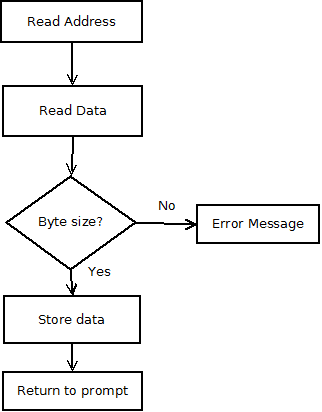
\includegraphics[width=0.7\linewidth]{MS}
\caption{Flowchart for Memory Set}
\label{fig:MS}
\end{figure}
			\paragraph{Assembly Code}~\\
			\lstinputlisting[firstnumber=986,firstline=986,lastline=1009]{Project.X68}
			
			\subsubsection{Block Fill}
			\paragraph{Algorithm and Flowchart}~\\
			This command requires two even addresses to be entered. It then parses the word sized data entered by the user and fills the block of memory from the first address to the second address. The syntax for this command is \texttt{BF <data> <address1> <address2>}. The flowchart is shown in Figure \ref{fig:BF}.
			
			
\begin{figure}[H]
\centering
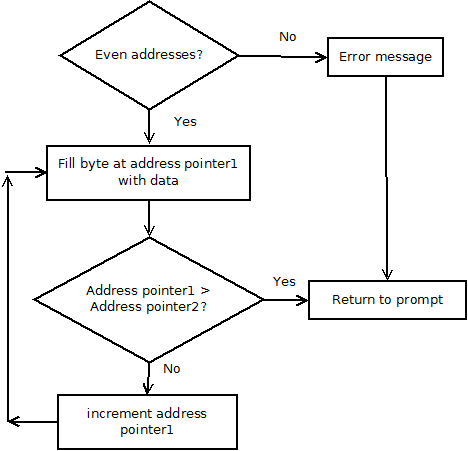
\includegraphics[width=0.7\linewidth]{BF}
\caption{Flowchart for Block Fill}
\label{fig:BF}
\end{figure}
			\paragraph{Assembly Code}~\\
			\lstinputlisting[firstnumber=1627,firstline=1627,lastline=1679]{Project.X68}
			
			\subsubsection{Block Move}
			
			
			
			\paragraph{Algorithm and Flowchart}~\\
			This command move a block of memory from one section to another. Both block sizes must be equal. Starting from the first address of the first block and the first address of the second block, it moves data byte by byte to the respective memory locations until all data has been copied. Its syntax is \texttt{BMOV <address1> <address2> <address3> <address4>}. The flowchart is shown in Figure \ref{fig:BMOV}.
			
\begin{figure}[H]
\centering
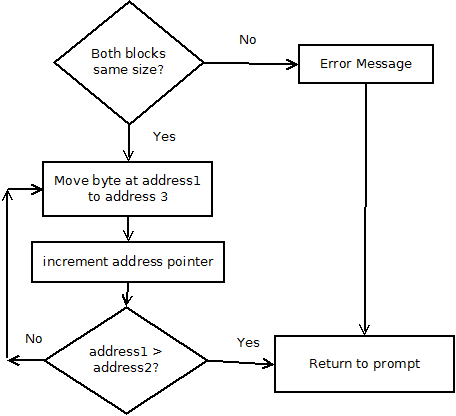
\includegraphics[width=0.7\linewidth]{BMOV}
\caption{Flowchart for Block Move}
\label{fig:BMOV}
\end{figure}
			\paragraph{Assembly Code}~\\				\lstinputlisting[firstnumber=1682,firstline=1682,lastline=1758]{Project.X68}
			
			\subsubsection{Block Test}
			\paragraph{Algorithm and Flowchart}~\\
			This command fills a block of memory with byte sized data, then checks each byte of the block. If any byte is not equal to the data originally written, the program outputs the data read and the address where the test failed. If no error is detected, the program outputs a message declaring the test passed. The syntax for this command is \texttt{BTST <data> <address1> <address2>}. The flowchart is shown in Figure \ref{fig:BTST}.
			
\begin{figure}[H]
\centering
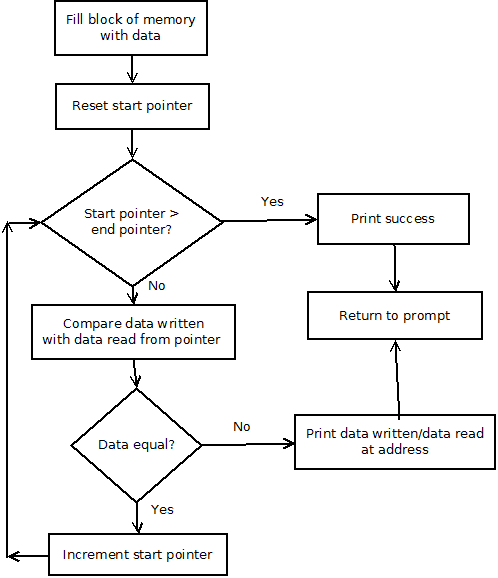
\includegraphics[width=0.7\linewidth]{BTST}
\caption{Flowchart for Block Test}
\label{fig:BTST}
\end{figure}
			
			\paragraph{Assembly Code}~\\				\lstinputlisting[firstnumber=1762,firstline=1762,lastline=1871]{Project.X68}
			
			\subsubsection{Block Search}
			
			\paragraph{Algorithm and Flowchart}~\\
			This command searches through a block of memory for data entered by the user. It does so by checking each value in memory byte by byte. The syntax for this command is \texttt{BSCH <data> <address1> <address2>}. The flowchart is shown in Figure \ref{fig:BSearch}.
			
			
			
\begin{figure}[H]
\centering
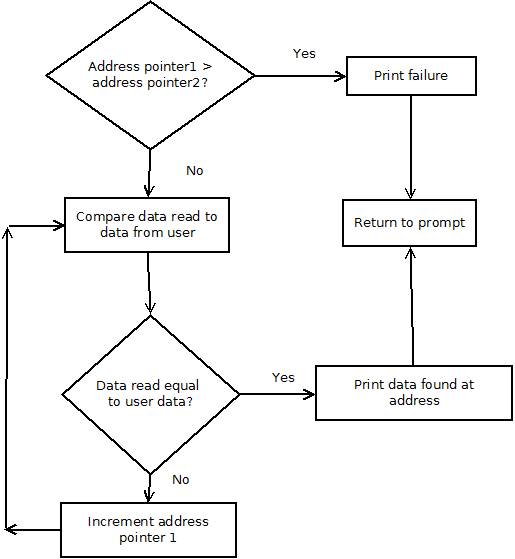
\includegraphics[width=0.7\linewidth]{BSearch}
\caption{Flowchart for Block Search}
\label{fig:BSearch}
\end{figure}
			\paragraph{Assembly Code}~\\				\lstinputlisting[firstnumber=1875,firstline=1875,lastline=1993]{Project.X68}
			
			\subsubsection{Go}
			
			\paragraph{Algorithm and Flowchart}~\\
			This command jumps to an address in memory and executes the machine code stored at that address. The syntax is \texttt{GO <address>}. The flowchart is shown in Figure \ref{fig:Go}.
			
			
\begin{figure}[H]
\centering
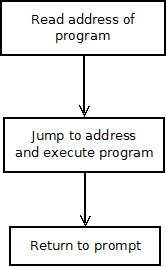
\includegraphics[width=0.2\linewidth]{Go}
\caption{Flowchart for Go}
\label{fig:Go}
\end{figure}
			\paragraph{Assembly Code}~\\				\lstinputlisting[firstnumber=1997,firstline=1997,lastline=2011]{Project.X68}
			
			\subsubsection{Display Formatted Registers}
		
			\paragraph{Algorithm and Flowchart}~\\
				This command displays the values of the registers as well as the stack pointers and program counter. It does so by first popping these values which were previously stored on stack item by item. They are then converted to ASCII for output and displayed on the terminal. The syntax is \texttt{DF}. The flowchart is shown in Figure \ref{fig:DF}.
			
			
\begin{figure}[H]
\centering
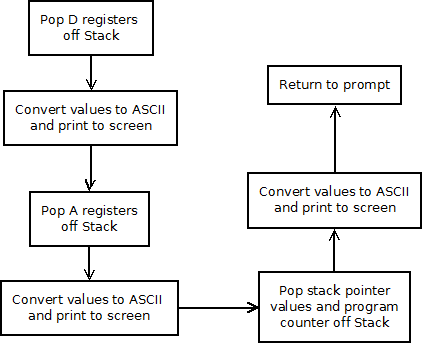
\includegraphics[width=0.7\linewidth]{DF}
\caption{Flowchart for Display Formatted Registers}
\label{fig:DF}
\end{figure}
			\paragraph{Assembly Code}~\\				\lstinputlisting[firstnumber=2015,firstline=2015,lastline=2419]{Project.X68}
			
			\subsubsection{Modify Register}
		
			\paragraph{Algorithm and Flowchart}~\\
				This command is used to change the value of a specific A or D register. This is done by parsing the data entered by the user, then updating the current value of the selected register. The syntax is \texttt{.<Register Type> <data>}. The flowchart is shown in Figure \ref{fig:ModifyReg}.
			
			
			
\begin{figure}[H]
\centering
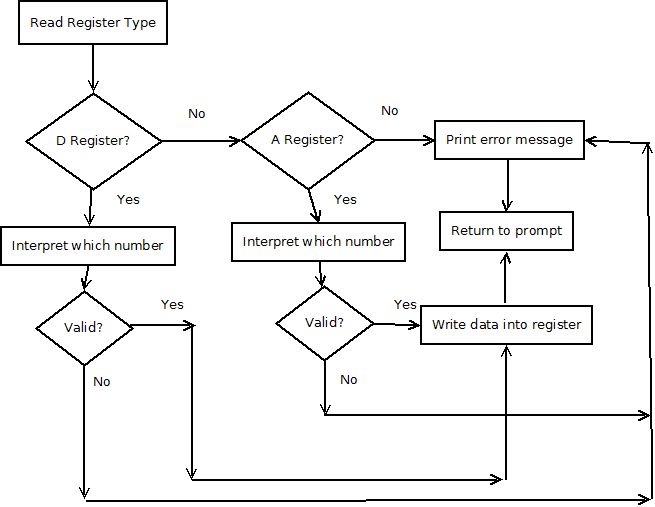
\includegraphics[width=0.7\linewidth]{ModifyReg}
\caption{Flowchart for Modify Register}
\label{fig:ModifyReg}
\end{figure}
			\paragraph{Assembly Code}~\\				\lstinputlisting[firstnumber=414,firstline=414,lastline=794]{Project.X68}
			
			\subsubsection{Echo}
			\paragraph{Algorithm and Flowchart}~\\
			This is a simple command that outputs what the user inputs. This is done by parsing the data entered by the user and immediately setting up a trap I/O call that outputs what was just entered. The syntax is \texttt{ECHO <data>}. The flowchart is shown in Figure \ref{fig:Echo}.
			\paragraph{Assembly Code}~\\				\lstinputlisting[firstnumber=399,firstline=399,lastline=412]{Project.X68}
		
			
\begin{figure}[H]
\centering
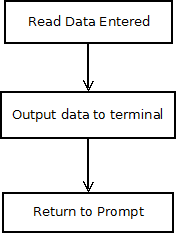
\includegraphics[width=0.3\linewidth]{Echo}
\caption{Flowchart for Echo}
\label{fig:Echo}
\end{figure}
			
			\subsection{Exception Handlers}
			The Monitor441 program uses custom exception handlers. They are loaded using the source code:
			\lstinputlisting[firstnumber=134,firstline=134,lastline=151]{Project.X68}
			\subsubsection{Bus Error Exception}
			\paragraph{Algorithm and Flowchart}~\\
			
			This exception is called whenever a bus error exception occurs. It outputs the SSW, IR, and BA along with a custom string message. The register values are also printed to the screen. The flowchart is shown in Figure \ref{fig:BERR}.
			
			
\begin{figure}[H]
\centering
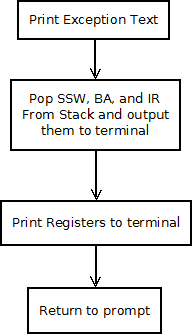
\includegraphics[width=0.3\linewidth]{BERR}
\caption{Flowchart for Bus Error Exception}
\label{fig:BERR}
\end{figure}
			\paragraph{Assembly Code}~\\				
			\lstinputlisting[firstnumber=2427,firstline=2427,lastline=2465]{Project.X68}
			
			
		
			\subsubsection{Address Error Exception}
			\paragraph{Algorithm and Flowchart}~\\
			This exception is called whenever an address error exception occurs. It outputs the SSW, IR, and BA along with a custom string message. The register values are also printed to the screen. The flowchart is shown in Figure \ref{fig:AERR}.
			
				\begin{figure}[H]
					\centering
					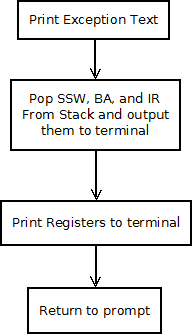
\includegraphics[width=0.3\linewidth]{BERR}
					\caption{Flowchart for Address Error Exception}
					\label{fig:AERR}
				\end{figure}
			\paragraph{Assembly Code}~\\			
				\lstinputlisting[firstnumber=2467,firstline=2467,lastline=2505]{Project.X68}
			
			\subsubsection{Illegal Instruction Error Exception}
			\paragraph{Algorithm and Flowchart}~\\
			This exception is called whenever an illegal instruction error exception occurs. It outputs a custom string message, and the register values are also printed to the screen. The flowchart is shown in Figure \ref{fig:Exception}.
			
\begin{figure}[H]
\centering
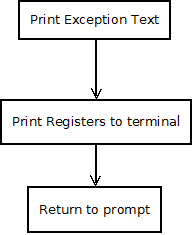
\includegraphics[width=0.3\linewidth]{Exception}
\caption{Flowchart for Illegal Instruction Exception}
\label{fig:Exception}
\end{figure}
			\paragraph{Assembly Code}~\\	
						\lstinputlisting[firstnumber=2507,firstline=2507,lastline=2514]{Project.X68}
			
			\subsubsection{Privilege Violation Error Exception}
			\paragraph{Algorithm and Flowchart}~\\
			This exception is called whenever an privilege violation error exception occurs. It outputs a custom string message, and the register values are also printed to the screen. The flowchart is shown in Figure \ref{fig:priv}.
			
			
\begin{figure}[H]
\centering
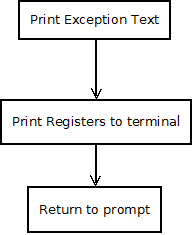
\includegraphics[width=0.3\linewidth]{Exception}
\caption{Flowchart for Privilege Violation Exception}
\label{fig:priv}
\end{figure}
			\paragraph{Assembly Code}~\\	
						\lstinputlisting[firstnumber=2516,firstline=2516,lastline=2523]{Project.X68}
			
			\subsubsection{Divide by Zero Error Exception}
			\paragraph{Algorithm and Flowchart}~\\
			This exception is called whenever a divide by zero error exception occurs. It outputs a custom string message, and the register values are also printed to the screen. The flowchart is shown in Figure \ref{fig:zero}.
			
			\begin{figure}[H]
				\centering
				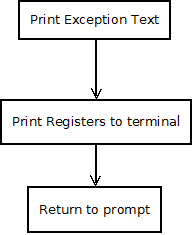
\includegraphics[width=0.3\linewidth]{Exception}
				\caption{Flowchart for Divide by Zero Exception}
				\label{fig:zero}
			\end{figure}
			\paragraph{Assembly Code}~\\	
						\lstinputlisting[firstnumber=2525,firstline=2525,lastline=2532]{Project.X68}
			
			\subsubsection{A Line Emulator Error Exception}
			\paragraph{Algorithm and Flowchart}~\\
			This exception is called whenever an A line emulator error exception occurs. It outputs a custom string message, and the register values are also printed to the screen. The flowchart is shown in Figure \ref{fig:Aline}.
			\begin{figure}[H]
				\centering
				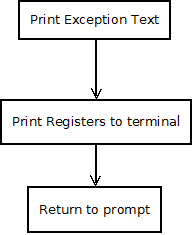
\includegraphics[width=0.3\linewidth]{Exception}
				\caption{Flowchart for A Line Emulator Error Exception}
				\label{fig:Aline}
			\end{figure}
			\paragraph{Assembly Code}~\\	
						\lstinputlisting[firstnumber=2534,firstline=2534,lastline=2541]{Project.X68}
			
			\subsubsection{F Line Emulator Error Exception}
			\paragraph{Algorithm and Flowchart}~\\
			This exception is called whenever an F line emulator error exception occurs. It outputs a custom string message, and the register values are also printed to the screen. The flowchart is shown in Figure \ref{fig:Fline}.
			
			\begin{figure}[H]
				\centering
				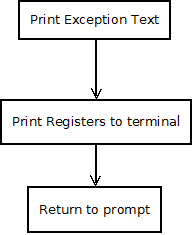
\includegraphics[width=0.3\linewidth]{Exception}
				\caption{Flowchart for F Line Emulator Error Exception}
				\label{fig:Fline}
			\end{figure}
			\paragraph{Assembly Code}~\\		
					\lstinputlisting[firstnumber=2543,firstline=2543,lastline=2551]{Project.X68}
			
			\subsubsection{Check Instruction Error Exception}
			\paragraph{Algorithm and Flowchart}~\\
			This exception is called whenever a check instruction error exception occurs. It outputs a custom string message, and the register values are also printed to the screen. The flowchart is shown in Figure \ref{fig:chk}.
			
			\begin{figure}[H]
				\centering
				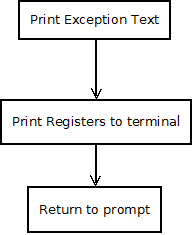
\includegraphics[width=0.3\linewidth]{Exception}
				\caption{Flowchart for Check Instruction Error Exception}
				\label{fig:chk}
			\end{figure}
			\paragraph{Assembly Code}~\\			
				\lstinputlisting[firstnumber=2553,firstline=2553,lastline=2561]{Project.X68}
			
			\subsection{User Instruction Manual Exception Handlers}
			
			\subsubsection{Syntax/Unknown Command Error}
			\paragraph{Algorithm and Flowchart}~\\
			This error is meant to guide the user to input the correct syntax for a command. It first checks if the command entered is valid. If not, an unknown command message is displayed. If the command entered is valid but the syntax is incorrect, an incorrect syntax message is outputted to the terminal. The flowchart is shown in Figure \ref{fig:UserInst}.
			
		
\begin{figure}[H]
\centering
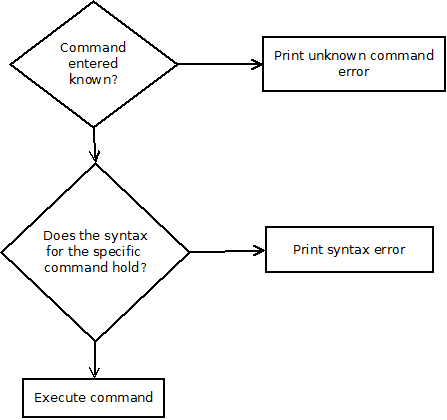
\includegraphics[width=0.7\linewidth]{UserInst}
\caption{Flowchart for User Instruction Manual Exception Handler}
\label{fig:UserInst}
\end{figure}
			\paragraph{Assembly Code}~\\
			\lstinputlisting[firstnumber=2569,firstline=2569,lastline=2573]{Project.X68}
			
			\lstinputlisting[firstnumber=2667,firstline=2667,lastline=2671]{Project.X68}
			
			
			\section{Discussion}\label{sec:discussion}
			With a low level programming language such as assembly, the computer engineer is in full control of how each command is built. When building a monitor type program, assembly can be great because of its simplicity, but it also has its draw backs due to a lack of high level API. This increases the chances that erroneous input will kill the program or produce unpredictable results. This means that in order to have a flawless program, the amount of source code needed to be written per command could easily violate the design constraint of having under 3K code size. Because of this, major errors were checked, but it is still possible to break the program by producing minor errors. The program assumes the user knows how to accurately use the tools provided, and if wrong input is entered and an error message is not displayed, the user will have already known their input was invalid. Furthermore, there are some major limitations to the functionality of this program, for example, certain commands can only take in byte sized data or a hexadecimal to decimal conversion can only accept a maximum value of FFFF. Regardless, this program performs on par with Motorola's Tutor software and, with error checking aside, could replace Tutor entirely. 
			
			There were many engineering and design challenges encountered during the journey to construct this program. A majority of these challenges came up during the debugging of each separate command. Taking an algorithm and knowing how to code it is a simple process, but the actual implementation is the hard part. This is when things such as runtime errors must be eliminated. Overall, runtime errors accounted for 95\% of the total generated errors, and the code had to be run step by step to pinpoint the exact moment of error in order to be fixed. Furthermore, deciding on how to store and manipulate data was a huge design concern. With only 7 data registers and 7 address registers, storage ``containers" had to be carefully picked so that there were no memory leaks and registers needed to be untouched due to subroutines were not accessed accidentally.
			\section{Feature Suggestions}
			As discussed earlier in Section \ref{sec:discussion}, complex error checking should be implemented in this program. Furthermore, more commands should be implemented to emulate not just Motorola's Tutor software, but current Operating System distributions as well. This could include commands such as , \texttt{ls} (listing files in current directory) or \texttt{cd} (change directory). If implementing an embedded system using the MC68000 processor, and the \texttt{MONITOR441} program is used as a basis, these commands could help the programmer easily analyze top layer applications such as installed files as well as low layer applications such as displaying register values.
			\section{Conclusion}
			Overall, the monitor program was created, and it has all of the requested functionality implemented. While it is not 100\% error free, it provides the user a great MC6000 based piece of software for use with debugging the microprocessor. Further work could be done to improve the functionality to be on the level of Motorola's Tutor software, but this shouldn't be done as no modern day technology runs based on the MC68000 microprocessor. 
			\begin{thebibliography}{1} 
				\bibitem{book}Harman, Thomas L., and Barbara Lawson. \emph{The Motorola MC68000 Microprocessor Family: Assembly Language, Interface Design, and System Design.} Englewood Cliffs, NJ: Prentice-Hall, 1985. Print. 
				\bibitem{manual} MC68000 Microprocessor Programmer's Reference Manual
				\bibitem{lab} SANPER-1 Lab Manuals
				\bibitem{edu} MC68000 Educational Computer Board User's Manual
			\end{thebibliography}
\end{document}